\documentclass[../main.tex]{subfiles}

\title{Capitolo 6 - Mirror Symmetry for Calabi-Yau varieties}
\author{Edoardo Manini}
\date{Marzo 17, 2025}

\begin{document}
\ifSubfilesClassLoaded{
\maketitle
\tableofcontents
}{}


Calabi-Yau 3-folds caught much attention from theoretical physics because they naturally appear in mathematical models for superstring theory. Physicists discovered a duality for Calabi-Yau 3-folds which is called Mirror Symmetry. This duality defines a correspondence between two topologically different Calabi-Yau 3-folds (”mirror partners”) $Y$ and $Y^\prime$
such that the Hodge numbers of $Y$ and $Y^\prime$ satisfy the relations 
\[
h^{1,1}(Y) = h^{2,1}(Y^\prime), \qquad  h^{1,1}(Y^\prime) = h^{2,1}(Y).
\]

In the paper of P. Candelas, X.C. de la Ossa, P.S. Green and L. Parkes \cite{COGP91} the Mirror Symmetry was applied to give predictions for the number of rational curves of any degree on general quintic 3-folds in $\PP^4$, which was conjectured to be finite by Clemens \cite{Cl84}. 
For degrees $\leq 3$ these predictions were confirmed by Katz \cite{Katz86} who also computed the number $609250$ of degree $2$ rational curves on a generic quintic 3-fold. The formula of \cite{COGP91} was proved by Givental \cite{Gi96}.

Here we are first going to describe the construction of Batyrev \cite{Bat94}, which gives a Mirror Symmetry for pais of Calaby-Yau varieties. 
The definition of a Calabi-Yau variety which we are going to use is the following, which allows certain types of singularities:
\begin{defn} \label{defnCalabiYau}
    A Calaby-Yau variety is a $d$-dimensional normal complex compact variety $Y$ which satisfies the following conditions:
    \begin{enumerate}
        \item $Y$ has at most Gorenstein canonical singularities.
        \item The canonical sheaf of $Y$ is trivial, i.e. $\Omega^d_Y \simeq \calO_Y$
        \item $H^1(Y,\calO_Y)= \cdots=H^{d-1}(Y,\calO_Y)=\{0\}$
    \end{enumerate}
\end{defn}
where a point of a normal complex variety is a \emph{Gorenstein canonical singularity} if $K_X$ is Cartier near the point and there is a local resolution of singularities $f \colon \tilde{Y} \to Y$ such that
\[
K_{\tilde{Y}} = f^*(K_Y)+ \sum_i a_i E_i
\]
where the sum is over all exceptional divisors $E_i$ of $f$ and $a_i \geq 0$ for all $i$.

Then we are going to use the mixed Hodge structure on the sheaf of vanishing cycles, constructed in \ref{MHSonvanishing}, to give a Mirror symmetry construction for pairs of Landau-Ginzburg models, following \cite{GKR17}.




\subsection{Toric Geometry}

We give a brief summary on toric geometry, which is essential to the construction of the Mirror pair of Calabi-Yau varieties as done by Batyrev.


Fix a lattice $N \simeq \Z^n$, define the real vector space $N_\RR = N \otimes_\Z \RR \simeq \RR^n$. Let also $M \defeq \Hom( N, \Z^n)$ and $M_\RR = M \otimes_\Z \RR$ be the dual lattice and vector space, that are naturally endowed with the standard pairing, that we
denote as $\langle \quad , \quad \rangle \colon M \times N \to \Z$.

\begin{defn}
A (strongly) convex polyhedral cone is a subset $\sigma = \left \{ \sum_{i=1}^s \lambda_i u_i | \lambda_i \geq 0 \right \} $ of $N_\RR$ where $u_1, \dots , u_s \in N_\RR$ (s.t. $\sigma \cap (-\sigma)= \{0\}$).
\end{defn} The vectors $u_1, \dots , u_s$, or equivalently the corresponding rays consisting of positive multiples of some $u_i$, are called generators for the cone $\sigma$. A convex polyhedral cone $\sigma$ is called rational if the generators are vectors in the lattice $N$. We will call \emph{cone} a rational strongly convex polyhedral cone. 
\begin{defn}
    A cone  $\sigma$ is called simplicial if the generators are linearly independent vectors over $\RR$.
\end{defn} 
We call dimension of $\sigma$, $\dim(\sigma)$, the dimension of the linear space spanned by  $\sigma +  (-\sigma)$. We define the dual of a cone: 
\[
\sigma^\vee = \{ u \in M_\RR | \langle u, v\rangle \geq 0 \quad \forall v \in \sigma \}.
\]
We can also define the orthogonal of a cone: $\sigma^\perp = \{ u \in M_\RR | \langle u, v \rangle = 0 \quad \forall v \in \sigma \}$.
We have that the dual of the dual of a cone is the cone itself: $(\sigma^\vee)^\vee= \sigma$. Moreover this duality operation reverses the order of inclusion, indeed if $\tau \subseteq \sigma$ are two cones we have $\tau^\vee \supseteq \sigma^\vee$. For a cone $    \sigma \subseteq N_\RR$, a face $\tau$ of $\sigma$ is a subset of $\sigma$ of the form $\tau = \sigma \cap u^\perp= \{ v \in \sigma | \langle u, v \rangle = 0 \}$ for some $u \in \sigma^\vee$. We call facets the faces of codimension 1. A face of a face is a face, and the intersection of two faces of is still a face. We have the
\begin{proposition} \textup{\cite[page 11]{Ful93}}
    The dual of a rational convex polyhedral cone is a rational convex polyhedral cone.
\end{proposition}


A \emph{fan} $\Sigma$ in $N_\RR$ is a finite set of cones (rational strongly convex polyhedral cones) $\sigma \subseteq N_\RR$ such that:
\begin{enumerate}
    \item each face of a cone in $\Sigma$ is a cone in $\Sigma$;
\item the intersection of two cones in $\Sigma$ is a face of each cone.
\end{enumerate}
We define the support of $\Sigma$ as $| \Sigma | = \bigcup_{ \sigma \in \Sigma} \sigma$ , and $\Sigma(d)$ as the set of $d$-dimensional cones in $\Sigma$, sometimes denoted as the $d$-skeleton of $\Sigma$.
The $1$-dimensional cones $\Sigma(1)$, also called rays, are specially important. We reserve the letter $\rho$ to stand for elements of $\Sigma(1)$. For each $\rho \in \Sigma(1)$, let $v_\rho$ be the unique generator of the semigroup $\rho \cap N$. Using these generators, a cone $\sigma \in \Sigma$ can be written
\[
\sigma = \left \{ \sum_{\rho \subset \sigma} \lambda_\rho v_\rho | \lambda_\rho \geq 0 \right \}.
\]
The $v_\rho$ are the generators of $\sigma$. A standard abuse of notation is to identify $\rho$ with $v_\rho$. Thus we may write $v_\rho \in \Sigma(1)$. If $r=| \Sigma(1)|$ is the number of $1$-dimensional cones, we sometimes denote the $v_\rho$'s by $v_1, \dots, v_r$.  
\begin{defn}
    A fan $\Sigma$ is simplicial if every cone  $\sigma$ in  $\Sigma$ is simplicial.
\end{defn}

\subsubsection{Toric varieties from fans}

\begin{defn}
From a fan $\Sigma$ we can define a toric variety denoted with $X_\Sigma$ as follows.
To each cone $\sigma$ in $\Sigma$ we associate the affine toric variety defined as
\[
X_\sigma = \Spec(\C[\sigma^\vee \cap M])
\]
where $\sigma^\vee \cap M$ is the subgroup of all lattice points in the dual cone and $\C[\sigma^\vee \cap M]$ is the $\C$-algebra with generators $\chi^m$, one for each $m \in \sigma^\vee \cap M$ and relations $\chi^m \chi^n = \chi^{m+n} $.
The toric variety associated to $\Sigma$ is given by the gluing of $X_\sigma$ for each $\sigma$ in $\Sigma$
\[
X_\Sigma = \bigsqcup_{\sigma \in \Sigma} X_\sigma / \sim  ,
\]
where we glue as follows: for any pair of cones $\sigma$, $\tau$ in $\Sigma$ the intersection $\sigma \cap \tau$ is a face of each, so
$X_{\sigma \cap \tau}$ is an open subvariety of both $X_\sigma$ and $X_\tau$, hence we glue along the immersion of the two open subvarieties.
\end{defn}
The fact that the resulting complex variety $X_\Sigma$ is Hausdorff (or the algebraic variety is separated) comes from the fact that if $\sigma $ and $\tau$ are cones intersecting in a common face, the diagonal map $X_{\sigma \cap \tau} \to X_\sigma \cap X_\tau$ is a closed embedding.

%insert examples here
%
%

Since the affine toric variety corrisponding to the trivial cone $\sigma=\{0\}$ is the torus $T_N = N \otimes \C^* = \Spec(\C[M]) = \Spec(\C[\sigma^\vee \cap M])$, we see that $T_N$ is an affine open subset of every toric variety $X_\Sigma$. The action of the torus on itself extends to an algebraic action of $T_N$ on $X_\Sigma$. This is where the name \emph{toric varieties} comes form.
Since the origin is a face for each cone in $\Sigma$, the torus $T_N$ is embedded in each open $X_\sigma$.

The torus action on $X_\Sigma$ has only finitely many orbits, and there is an inclusion-reversing one-to-one correspondence between orbit closures and cones of $\Sigma$. In particular, each $\rho \in \Sigma(1) $ correspond to an irreducible $T_N$-invariant (Weil) divisor $D_\rho \subset X_\Sigma$. Furthermore, $m \in M$ gives a character $\chi^m \colon T_N \to \C^*$, and regarding $\chi^m$ as a rational function on $X_\Sigma$, we have
\begin{equation}\label{divcar}
    \divis(\chi^m)= \sum_{\rho \in \Sigma(1)} \langle m, v_\rho \rangle D_\rho.
\end{equation}
The properties of the fan  $\Sigma$ strongly affect the geometry of the toric variety $X_\Sigma$. For example:
\begin{enumerate}
    \item $X_\Sigma$ is compact if and only if $| \Sigma | = N_\RR$, such a fan is called complete.
    \item $X_\Sigma$ is smooth if and only if for every cone in $\Sigma$, its generators are part of a $\Z$-basis of $N$.
    \item $X_\Sigma$ is an orbifold if and only if $\Sigma$ is simplicial.
    \end{enumerate}

    The notion of an orbifold was introduced in \cite{Thu97}. For us an orbifold is an $n$-dimensional variety $X$ s.t. for every $p \in X$, there is a neighborhood analytically equivalent to $U/G \ni 0$, where $G \subset \GL (n,\C)$ is a finite subgroup with no complex reflections other than the identity and $U \subset \C^n$ is a $G$-stable neighborhood of the origin.

    In this definition, a \emph{complex reflection} is an element of $\GL (n,\C)$ of finite order such that $n-1$ of its eigenvalues are equal to 1.
    
The Chow group $A_{n-1}(X)$ of $(n-1)$-dimensional cycles, i.e. the Weil divisors modulo linear equivalence can be computed directly from the fan, assuming the 1-dimensional cones span $N_\RR$, which we will do. If we let $X=X_\Sigma$ and $\Div_T(X)$ be the group of $T_N$-invariant Weil divisors, using (\ref{divcar}), we get an exact sequence
\begin{equation}
    0 \lra M \lra \ZZ^{\Sigma(1)}=Div_T(X) \lra A_{n-1}(X) \lra 0
\end{equation}
where $m \in M$ maps to $\divis (\chi^m) \in \ZZ^{\Sigma(1)}$ and $(a_\rho) \in \Z^{\Sigma(1)}$ maps to the divisor class of $\sum_\rho (a_\rho)D_\rho $. Thus $A_{n-1}(X)$ has rank $r-n$.

Recall that a Cartier divisor is given by a section of $\calM_X^\times / \calO_X^\times $, i.e. a collection of $\{U_i,f_i \}$, where $\{U_i\}$ is an open cover of $X$, and the $f_i$ are rational functions on $U_i$ such that $f_i / f_j \in \calO_X^\times(U_i \cap U_j)$. Then for all codimension-1 subvarieties $Z$, $\ord_Z(f_i / f_j)=0$, hence $\ord_Z(f_i)=\ord_Z(f_j) \eqdef \ord_Z(D)$ . Every Cartier divisor $D$ determines a Weil divisor
\[
[D] = \sum_{\codim_X(V )=1} \ord_V (D) \cdot V.
\]
On smooth varieties Weil and Cartier divisors coincide, but this is not the case in the general setting. We will only consider divisors that are invariant under the action of the torus. We have a condition on toric varieties for a Weil divisor to be Cartier. 
\begin{proposition} \textup{\cite[Thm. 4.2.8]{CLS11}} \label{CartierWeil}
    A Weil divisor $D = \sum_{\rho} a_\rho D_\rho$ is Cartier if and only if for each $\sigma \in \Sigma $, there is $u_\sigma \in M$ such that $\langle u_\sigma , v_\rho \rangle = -a_\rho$ whenever $\rho \subset \sigma$.
\end{proposition}

Given a Cartier divisor $D$, we can define a piecewise linear function
$\phi_D \colon |\Sigma| \to \RR$, defined by $\phi_D(v) = \langle u_\sigma, v \rangle \quad \forall v \in \sigma$.
This function, called the \emph{support function} of $D$, is well defined and continuous, and clearly piecewise linear.
Vice versa if the fan $\Sigma$ is simplicial, meaning the generators of every cone in the fan are linearly independent over $\RR$, any continuous function on $|\Sigma|$ that is linear and integral on each cone $\sigma$ is induced by a Cartier divisor. This can be seen since, given a divisor $D = \sum_i a_i D_i$ the function $\phi_D$ is defined by $\phi_D(v_i) = -a_i$ , and we have $[D] = \sum_i -\phi_D(v_i) D_i$.

\subsubsection{Toric varieties from polytopes}

   \begin{defn}
       A convex \emph{polytope} $\Delta$ in a finite dimensional vector space $M_\RR$ is the convex hull of a finite set of points.
   \end{defn}  The \emph{dimension} of $\Delta$ is the dimension of the subspace spanned by the differences $\{ m_1 - m_2 | m_1,m_2 \in \Delta\}$. We say that $\Delta$ is a lattice (or integral) polytope if the vertices of $\Delta$ lie in $M$ (equivalently, $\Delta$ is the convex hull of a finite subset of $M$). A face is $F = \{ u \in \Delta | \langle u, v_F \rangle = a_F \}$, where $v_F \in N_\RR$ and $\langle u, v_F\rangle \geq a_F \quad \forall u \in \Delta$. We call the halfspace defined
by this equation the \emph{supporting halfspace} for the face.
A polytope can be written as the intersection of supporting halfspaces for all faces. Vice versa any bounded intersection of halfspaces gives rise to a polytope.
Finally, a facet is a codimension one face of $\Delta$.

Polytopes arise naturally when dealing with toric varieties.


For example, a Cartier divisor $D = \sum_i a_i D_i$ on $X_\Sigma$ determines a polyhedron $\Delta_D \subset M_\RR$:
\begin{align*}
\Delta_D &= \{ m \in M_\RR | \langle m, v \rangle \geq \phi_D(v) \quad \forall v \in |\Sigma| \}  \\ &= \{ u \in M_\RR | \langle u, v_i \rangle \geq -a_i \quad \forall i \} 
\end{align*}
where the $v_i$'s are the rays of the fan $\Sigma$.
We say that $\Delta_D$ is a polyhedron since it is an intersection of finitely many closed half spaces. A polytope is a bounded polyhedron.


\begin{lemma} \textup{\cite[Prop. 4.3.3]{CLS11}}
    Let $D = \sum_i a_i D_i$ be a Cartier divisor on $X=X_\Sigma$, then the global sections of the line bundle $\calO_X(D)$ are generated by the lattice points in $\Delta_D$, that is
    \[
    H^0(X,\calO(D)) \simeq \bigoplus_{m \in \Delta_D \cap M} \CC \cdot {\chi^m}. 
    \]
\end{lemma} 
\begin{proof}
    Recall that we define $\calO(D)$ to be the invertible fractional ideal sheaf defined by $D$, i.e. a sub-$\calO_X$-module of $\calM_X$, the sheaf of rational functions on $X$, which is locally free when $X$ is smooth. In particular, for $U \subset X$ an open, 
    \[
    \calO(D)(U) \defeq \{ f \in \calM_X(U) | \divis(f) \geq -D \text{ on } U \} \cup \{0\}.
    \]
     If $f \in \Gamma(X_\Sigma,\calO_{X_\Sigma}(D))$, then $\divis(f) + D \geq 0$ implies $\divis(f)|_{T_N} \geq 0$ since $D|_{T_N} = 0$. Since $\CC[M]$ is the coordinate ring of $T_N$, we have $f \in \CC[M]$. Thus
     \[
     H^0(X_\Sigma,\calO_{X_\Sigma}(D)) \subseteq \CC[M].
     \]
Furthermore, $H^0(X_\Sigma,\calO_{X_\Sigma}(D))$ is invariant under the $T_N$-action on $\CC[M]$ since $D$ is $T_N$-invariant. We obtain
\[
H^0(X_\Sigma,\calO_{X_\Sigma}(D)) = \bigoplus_{\chi^m \in H^0(X_\Sigma,\calO_{X_\Sigma}(D))} \CC \cdot \chi^m.
\]
Since $\chi^m \in \Gamma(X_\Sigma,\calO_{X_\Sigma}(D))$ if and only if $\divis(\chi^m) +D \geq 0$, or equivalently
\[
\langle m,u_\rho \rangle \geq -a_\rho \quad \text{ for all } \rho \in \Sigma(1),
\]
we are done.
\end{proof}




Consider a basis $\{ f_1,\dots , f_r \}$ of $\Gamma(X_\Sigma,\calO(D))$, defining $Bl(D)= \bigcap\limits_{D_{eff} \in |D|} Supp(D_{eff}) $ as the base locus, we can define
the following map:
\begin{align*}
\psi_D \colon X_\Sigma \setminus Bl(D) &\to \PP^{r-1} \\
x &\mapsto (f_1(x) : \cdots : f_r(x))
\end{align*}
so when the divisor $D$ is basepoint free, the map $\psi_D$ is a map $X_\Sigma \to \PP^{r-1}$. We know that a basis for $\calO(D)$ is given by $\{ \chi^{u_i} | u_i \in \Delta_D \cap M \}$, so choosing an ordering of the points in $\Delta_D \cap M$ gives us a mapping to the projective space:
\begin{align*}
\psi_D \colon X_\Sigma &\to \PP^{r-1} \\
x &\mapsto (f_1(x) : \cdots : f_r(x))
\end{align*}
We say that $D$ is very ample if this map is an embedding. We say that $D$ is ample if there exists $m >0$ s.t. $mD$ is very ample.
There is a criterion relating the ampleness of $D$ and the geometry of $\Delta_D$. Namely we have that $D$ is ample if and only if $\Delta_D$ is full dimensional.


%insert here examples of polytopes
%
%


If $\Delta \subset M_\RR$ is full dimensional and contains the origin in its interior, we can define the polar polytope of $\Delta$ as $\Delta^\circ = \{ v \in N_\RR | \langle m, v\rangle \geq -1 \quad \forall m \in \Delta \} \subset N_\RR$.
The polar polytope $\Delta^\circ$ is a convex polytope, it also contains the origin as an interior point and  $\Delta =  (\Delta^\circ)^\circ$. For every face $F$ of $\Delta$ we define the polar face $F^\circ= \{v \in \Delta^\circ | \langle u, v\rangle = -1 \quad \forall u \in F \}$ of $\Delta^\circ$.
We have an alternative characterization of the polar polytope. For each facet $F$ of $\Delta$ we have the supporting halfspace defined by the equation $\langle v, u_F \rangle \geq -a_F$ . Since the origin is in the interior of $\Delta$ we must have that $a_F$ are all positive. Then we have that the polar polytope is given by
\begin{equation} \label{reflpol}
\Delta^\circ = \Conv \left\{\frac{1}{a_F} u_F | F \text{ is a face of } \Delta \right\} .
\end{equation}


Consider now a lattice polytope $\Delta$ in the space $M_\RR$. If $\Delta$ is of maximal dimension we can associate a fan $\Sigma_\Delta$ to $\Delta$, called the the normal fan. For every face $F$ of $\Delta$ we define the cone $\sigma_F = \{ v \in N_\RR | \langle u, v\rangle \leq \langle u^\prime, v \rangle \quad \forall u \in F, u^\prime \in \Delta \}$. If $F$ is a facet, $\sigma_F$ is the ray generated by $u_F$. If $F$ is a vertex, $\sigma^\vee_F$ is the cone corresponding to the angle at $F$. The cones $\sigma_F$, where $F$ varies over all \emph{faces} of $\Delta$, form a fan, that we call normal fan and denote $\Sigma_\Delta$.
%
%
%
%insert here picture of normal fan
%
%

\begin{defn}
    Given $\Delta$ in $M_\RR$ a lattice polytope of maximal dimension, we call the toric variety associated to $\Delta$ the toric variety $X_\Delta \defeq X_{\Sigma_\Delta}$ associated to the normal fan of $\Delta$.
\end{defn} 

Notice that, since the normal fan of a lattice polytope is always complete, the associated toric variety $X_\Delta$ is always compact.

\begin{proposition} \label{normalfan}
    If $\Delta$ is a full dimensional lattice polytope in $M_\RR$ s.t. $0 \in \Int \Delta$, then the normal fan $\Sigma_\Delta$ is the fan consisting of cones over the faces of $\Delta^\circ$.
\end{proposition} 
% also Lemma 3.2.1 Cox and Katz
\begin{proof}
Since the normal fan $\Sigma_\Delta$ is given by the cones  \[
\sigma_F = \{ v \in N_\RR | \langle u, v\rangle \leq \langle u^\prime, v \rangle \quad \forall u \in F, u^\prime \in \Delta \}
\]
for every face $F$ of $\Delta$, we need to show that 
\[
\sigma_F = \{ \lambda v | v \in F^\circ, \lambda \geq 0 \}.
\]
First, if $v \in F^\circ \subset \Delta^\circ$, then $\forall u \in F$, $\langle u, v \rangle = -1$ by definition of $F^\circ$ and  $\forall u^\prime \in \Delta$, $\langle u^\prime, v \rangle \geq -1$ by definition of $\Delta^\circ$. Hence $\langle u,v \rangle \leq \langle u^\prime,v \rangle $, which implies
\[
\langle u^\prime , \lambda v \rangle = \lambda \langle u^\prime, v \rangle \geq  \lambda \langle u, v \rangle = \langle  u, \lambda v \rangle \quad \forall\lambda\geq 0,
\]
i.e. $\lambda v \in \sigma_F$.
For the other inclusion, let $v \in \sigma_F$. WLOG $v \neq 0$, this implies $\langle u, v \rangle < 0 \quad \forall u \in F$, since otherwise we would have $\forall u^\prime \in \Delta$, $\langle u^\prime, v \rangle \geq 0$ which would imply $0 \in \partial \Delta$, which is not possible since $0 \in \Int \Delta$.
Fix $u$ in $F$, then $\langle u, v \rangle \defeq -\lambda < 0$ for some $\lambda >0$. Setting $v=\lambda v^\prime$, we have $\langle u^\prime, v^\prime \rangle \geq \langle u, v^\prime \rangle = -1 ,\quad \forall u^\prime \in \Delta, \forall u \in F$. This implies $v^\prime \in \Delta^\circ$ and $v^\prime \in F^\circ$.
    %See also \cite[p. 26]{Ful93}.
\end{proof}

To conclude the section we explain how a toric variety $X_\Delta$ coming from a polytope $\Delta$ comes always with a choice of an ample Cartier divisor, hence an ample line bundle. Indeed, on $X_\Delta$ we have a divisor $ D_\Delta$ defined by the convex function $\phi_\Delta \colon N_\RR \to \RR$ defined by
\[
\phi_\Delta(v) = \min_{u \in \Delta} \langle u, v \rangle = \min_i \langle u_i, v \rangle,
\]
where $u_i$ are the vertices of $\Delta$. 
One can show that $\Delta = \Delta_{D_\Delta}$ and $D=D_\Delta$ is very ample, hence we have an embedding of the variety in a projective space with a specific choice of an ample divisor. We will denote $\calO_{X_\Delta}(1) \defeq \calO_{X_\Delta}(D_{\Delta}) $.

Conversely if we start from an ample divisor $D$ on a toric variety $X_{\Sigma}$, then $\Sigma$ is the normal fan of $\Delta_D$.
The previous discussion proves that a toric variety $X_{\Sigma}$ is projective if and only if the fan $\Sigma$ is the normal fan of a convex polytope. We summarize this in the following

\begin{theorem} \textup{\cite[Thm. 6.2.1]{CLS11}}
    There is a bijection
    \begin{align*}
 \left\{ \Delta \subset M_\RR \ \middle\vert \begin{array}{l}
     \Delta \textrm{ is a full dimensional } \\
    \textrm{lattice polytope }
  \end{array}\right\} &\longleftrightarrow  \left\{ (X_\Sigma,D) \ \middle\vert \begin{array}{l}
     \Sigma \text{ a complete fan in } N_\RR, \\
    D \text{ a torus-invariant } \\ 
   \text{ample divisor on } X_\Sigma
  \end{array}\right\} \\
\Delta &\longmapsto (X_\Delta, D_\Delta) \\
\Delta_D &\longmapsfrom (X_\Sigma,D) 
    \end{align*}

\end{theorem}

%inserire qui esempio cubo stortato: not every fan is the normal fan of a polytope.

Indeed, the varieties we are going to introduce in next section are all going to be projective.




\subsubsection{Fano varieties from reflexive polytopes}


In general the polar of an integral polytope is not an integral polytope, to guarantee this we have to introduce the notion of reflexive polytopes of Batyrev. This is crucial for the mirror symmetry construction.
\begin{defn}
    A $n$-dimensional integral polytope $\Delta \subset M_\RR$ is reflexive if all facets of $\Delta$ are supported by an affine halfspace of the form $ \{ m \in M_\RR | \langle m, v\rangle \geq -1 \}$ for some vector $v \in N$. 
\end{defn} 

\begin{figure}[!ht] 
    \centering
    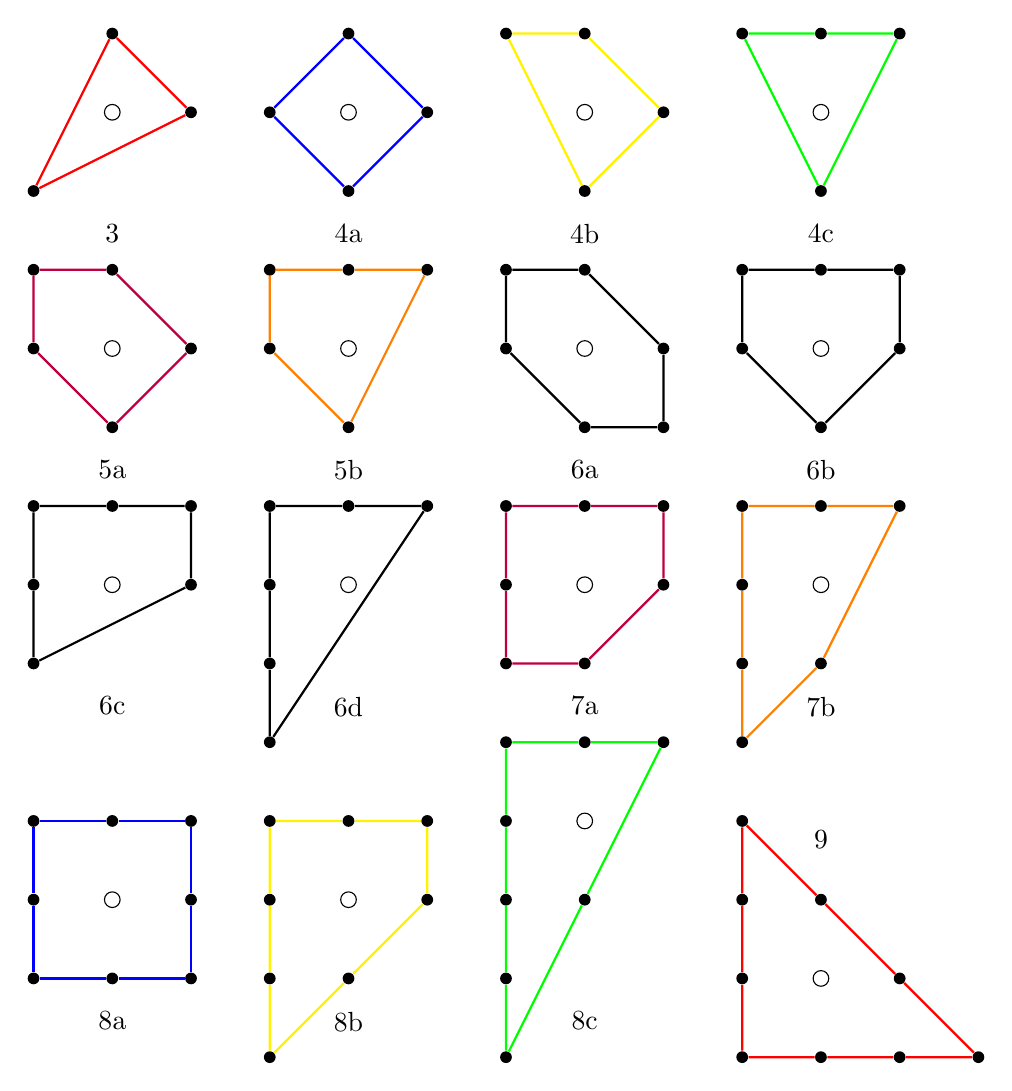
\begin{tikzpicture}[scale=1]

    % Polygon 3
    \begin{scope}[shift={(0,4)}]
        \node[circle, fill=black, inner sep=1.5pt] (3-1) at (0,1) {};
        \node[circle, fill=black, inner sep=1.5pt] (3-2) at (1,0) {};
        \node[circle, fill=black, inner sep=1.5pt] (3-3) at (-1,-1) {};
        \node[circle, draw=black, inner sep=2pt] at (0,0) {};
        \draw[red,thick] (3-1) -- (3-2) -- (3-3) -- (3-1);
        \node[below=0.3cm] at (0,-1) {3};
    \end{scope}

    % Polygon 4a
    \begin{scope}[shift={(3,4)}]
        \node[circle, fill=black, inner sep=1.5pt] (4a-1) at (1,0) {};
        \node[circle, fill=black, inner sep=1.5pt] (4a-2) at (0,1) {};
        \node[circle, fill=black, inner sep=1.5pt] (4a-3) at (-1,0) {};
        \node[circle, fill=black, inner sep=1.5pt] (4a-4) at (0,-1) {};
        \node[circle, draw=black, inner sep=2pt] at (0,0) {};
        \draw[blue,thick] (4a-1) -- (4a-2) -- (4a-3) -- (4a-4) -- (4a-1);
        \node[below=0.3cm] at (0,-1) {4a};
    \end{scope}

    % Polygon 4b
    \begin{scope}[shift={(6,4)}]
        \node[circle, fill=black, inner sep=1.5pt] (4b-1) at (1,0) {};
        \node[circle, fill=black, inner sep=1.5pt] (4b-2) at (0,-1) {};
        \node[circle, fill=black, inner sep=1.5pt] (4b-3) at (-1,1) {};
        \node[circle, fill=black, inner sep=1.5pt] (4b-4) at (0,1) {};
        \node[circle, draw=black, inner sep=2pt] at (0,0) {};
        \draw[yellow,thick] (4b-1) -- (4b-2) -- (4b-3)  -- (4b-4) -- (4b-1);
        \node[below=0.3cm] at (0,-1) {4b};
    \end{scope}
    
    % Polygon 4c
    \begin{scope}[shift={(9,4)}]
        \node[circle, fill=black, inner sep=1.5pt] (4c-1) at (1,1) {};
        \node[circle, fill=black, inner sep=1.5pt] (4c-2) at (0,-1) {};
        \node[circle, fill=black, inner sep=1.5pt] (4c-3) at (-1,1) {};
        \node[circle, fill=black, inner sep=1.5pt] (4c-4) at (0,1) {};
        \node[circle, draw=black, inner sep=2pt] at (0,0) {};
        \draw[green,thick] (4c-1) -- (4c-2) -- (4c-3) -- (4c-4) -- (4c-1);
        \node[below=0.3cm] at (0,-1) {4c};
    \end{scope}

    % Polygon 5a
   \begin{scope}[shift={(0,1)}]
        \node[circle, fill=black, inner sep=1.5pt] (5a-1) at (0,1) {};
        \node[circle, fill=black, inner sep=1.5pt] (5a-2) at (1,0) {};
        \node[circle, fill=black, inner sep=1.5pt] (5a-3) at (0,-1) {};
        \node[circle, fill=black, inner sep=1.5pt] (5a-4) at (-1,0) {};
        \node[circle, fill=black, inner sep=1.5pt] (5a-5) at (-1,1) {};
        \node[circle, draw=black, inner sep=2pt] at (0,0) {};
        \draw[purple,thick] (5a-1) -- (5a-2) -- (5a-3) -- (5a-4) -- (5a-5) -- (5a-1);
        \node[below=0.3cm] at (0,-1) {5a};
    \end{scope}

    % Polygon 5b
    \begin{scope}[shift={(3,1)}]
        \node[circle, fill=black, inner sep=1.5pt] (5b-1) at (-1,1) {};
        \node[circle, fill=black, inner sep=1.5pt] (5b-2) at (0,1) {};
        \node[circle, fill=black, inner sep=1.5pt] (5b-3) at (1,1) {};
        \node[circle, fill=black, inner sep=1.5pt] (5b-4) at (0,-1) {};
         \node[circle, fill=black, inner sep=1.5pt] (5b-5) at (-1,0) {};
        \node[circle, draw=black, inner sep=2pt] at (0,0) {};
        \draw[orange,thick] (5b-1) -- (5b-2) -- (5b-3) -- (5b-4) -- (5b-5) --(5b-1);
        \node[below=0.3cm] at (0,-1) {5b};
    \end{scope}

    % Polygon 6a
    \begin{scope}[shift={(6,1)}]
        \node[circle, fill=black, inner sep=1.5pt] (6a-1) at (1,0) {};
        \node[circle, fill=black, inner sep=1.5pt] (6a-2) at (0,1) {};
        \node[circle, fill=black, inner sep=1.5pt] (6a-3) at (-1,1) {};
        \node[circle, fill=black, inner sep=1.5pt] (6a-4) at (-1,0) {};
        \node[circle, fill=black, inner sep=1.5pt] (6a-5) at (0,-1) {};
        \node[circle, fill=black, inner sep=1.5pt] (6a-6) at (1,-1) {};
        \node[circle, draw=black, inner sep=2pt] at (0,0) {};
        \draw[thick] (6a-1) -- (6a-2) -- (6a-3) -- (6a-4) -- (6a-5) --(6a-6) --(6a-1);
        \node[below=0.3cm] at (0,-1) {6a};
    \end{scope}

    % Polygon 6b
   \begin{scope}[shift={(9,1)}]
        \node[circle, fill=black, inner sep=1.5pt] (6b-1) at (1,1) {};
        \node[circle, fill=black, inner sep=1.5pt] (6b-2) at (0,1) {};
        \node[circle, fill=black, inner sep=1.5pt] (6b-3) at (-1,1) {};
        \node[circle, fill=black, inner sep=1.5pt] (6b-4) at (-1,0) {};
        \node[circle, fill=black, inner sep=1.5pt] (6b-5) at (0,-1) {};
        \node[circle, fill=black, inner sep=1.5pt] (6b-6) at (1,0) {};
        \node[circle, draw=black, inner sep=2pt] at (0,0) {};
        \draw[thick] (6b-1) -- (6b-2) -- (6b-3) -- (6b-4) -- (6b-5) -- (6b-6) -- (6b-1);
        \node[below=0.3cm] at (0,-1) {6b};
    \end{scope}
%\vspace{2px}
    % Polygon 6c
    \begin{scope}[shift={(0,-2)}]
        \node[circle, fill=black, inner sep=1.5pt] (6c-1) at (1,1) {};
        \node[circle, fill=black, inner sep=1.5pt] (6c-2) at (0,1) {};
        \node[circle, fill=black, inner sep=1.5pt] (6c-3) at (-1,1) {};
        \node[circle, fill=black, inner sep=1.5pt] (6c-4) at (-1,0) {};
        \node[circle, fill=black, inner sep=1.5pt] (6c-5) at (-1,-1) {};
        \node[circle, fill=black, inner sep=1.5pt] (6c-6) at (1,0) {};
        \node[circle, draw=black, inner sep=2pt] at (0,0) {};
        \draw[thick] (6c-1) -- (6c-2) -- (6c-3) -- (6c-4) -- (6c-5) -- (6c-6) -- (6c-1);
        \node[below=0.3cm] at (0,-1) {6c};
    \end{scope}

    % Polygon 6d
    \begin{scope}[shift={(3,-2)}]
        \node[circle, fill=black, inner sep=1.5pt] (6d-1) at (1,1) {};
        \node[circle, fill=black, inner sep=1.5pt] (6d-2) at (0,1) {};
        \node[circle, fill=black, inner sep=1.5pt] (6d-3) at (-1,1) {};
        \node[circle, fill=black, inner sep=1.5pt] (6d-4) at (-1,0) {};
        \node[circle, fill=black, inner sep=1.5pt] (6d-5) at (-1,-1) {};
        \node[circle, fill=black, inner sep=1.5pt] (6d-6) at (-1,-2) {};
        \node[circle, draw=black, inner sep=2pt] at (0,0) {};
        \draw[thick] (6d-1) -- (6d-2) -- (6d-3) -- (6d-4) -- (6d-5) -- (6d-6) -- (6d-1);
        \node[below=0.3cm] at (0,-1) {6d};
    \end{scope}

    % Polygon 7a
    \begin{scope}[shift={(6,-2)}]
        \node[circle, fill=black, inner sep=1.5pt] (7a-1) at (1,1) {};
        \node[circle, fill=black, inner sep=1.5pt] (7a-2) at (0,1) {};
        \node[circle, fill=black, inner sep=1.5pt] (7a-3) at (-1,1) {};
        \node[circle, fill=black, inner sep=1.5pt] (7a-4) at (-1,0) {};
        \node[circle, fill=black, inner sep=1.5pt] (7a-5) at (-1,-1) {};
        \node[circle, fill=black, inner sep=1.5pt] (7a-6) at (0,-1) {};
        \node[circle, fill=black, inner sep=1.5pt] (7a-7) at (1,0) {};
        \node[circle, draw=black, inner sep=2pt] at (0,0) {};
        \draw[purple,thick] (7a-1) -- (7a-2) -- (7a-3) -- (7a-4) -- (7a-5) -- (7a-6) -- (7a-7) -- (7a-1);
        \node[below=0.3cm] at (0,-1) {7a};
    \end{scope}

    % Polygon 7b
    \begin{scope}[shift={(9,-2)}]
        \node[circle, fill=black, inner sep=1.5pt] (7b-1) at (1,1) {};
        \node[circle, fill=black, inner sep=1.5pt] (7b-2) at (0,1) {};
        \node[circle, fill=black, inner sep=1.5pt] (7b-3) at (-1,1) {};
         \node[circle, fill=black, inner sep=1.5pt] (7b-4) at (-1,0) {};
         \node[circle, fill=black, inner sep=1.5pt] (7b-5) at (-1,-1) {};
         \node[circle, fill=black, inner sep=1.5pt] (7b-6) at (-1,-2) {};
         \node[circle, fill=black, inner sep=1.5pt] (7b-7) at (0,-1) {};
        \node[circle, draw=black, inner sep=2pt] at (0,0) {};
        \draw[orange,thick] (7b-1) -- (7b-2) -- (7b-3) -- (7b-4) -- (7b-5) -- (7b-6) -- (7b-7) -- (7b-1);
        \node[below=0.3cm] at (0,-1) {7b};
    \end{scope}

    % Polygon 8a
    \begin{scope}[shift={(0,-6)}]
        \node[circle, fill=black, inner sep=1.5pt] (8a-1) at (1,1) {};
        \node[circle, fill=black, inner sep=1.5pt] (8a-2) at (0,1) {};
        \node[circle, fill=black, inner sep=1.5pt] (8a-3) at (-1,1) {};
        \node[circle, fill=black, inner sep=1.5pt] (8a-4) at (-1,0) {};
        \node[circle, fill=black, inner sep=1.5pt] (8a-5) at (-1,-1) {};
        \node[circle, fill=black, inner sep=1.5pt] (8a-6) at (0,-1) {};
        \node[circle, fill=black, inner sep=1.5pt] (8a-7) at (1,-1) {};
        \node[circle, fill=black, inner sep=1.5pt] (8a-8) at (1,0) {};
        \node[circle, draw=black, inner sep=2pt] at (0,0) {};
        \draw[blue,thick] (8a-1) -- (8a-2) -- (8a-3) -- (8a-4) -- (8a-5) -- (8a-6) -- (8a-7) -- (8a-8) -- (8a-1);
        \node[below=0.3cm] at (0,-1) {8a};
    \end{scope}

    % Polygon 8b
    \begin{scope}[shift={(3,-6)}]
        \node[circle, fill=black, inner sep=1.5pt] (8b-1) at (1,1) {};
        \node[circle, fill=black, inner sep=1.5pt] (8b-2) at (0,1) {};
        \node[circle, fill=black, inner sep=1.5pt] (8b-3) at (-1,1) {};
        \node[circle, fill=black, inner sep=1.5pt] (8b-4) at (-1,0) {};
        \node[circle, fill=black, inner sep=1.5pt] (8b-5) at (-1,-1) {};
        \node[circle, fill=black, inner sep=1.5pt] (8b-6) at (-1,-2) {};
        \node[circle, fill=black, inner sep=1.5pt] (8b-7) at (0,-1) {};
        \node[circle, fill=black, inner sep=1.5pt] (8b-8) at (1,0) {};
        \node[circle, draw=black, inner sep=2pt] at (0,0) {};
        \draw[yellow,thick] (8b-1) -- (8b-2) -- (8b-3) -- (8b-4) -- (8b-5) -- (8b-6) -- (8b-7) -- (8b-8) -- (8b-1);
        \node[below=0.3cm] at (0,-1) {8b};
    \end{scope}

    % Polygon 8c
    \begin{scope}[shift={(6,-5)}]
        \node[circle, fill=black, inner sep=1.5pt] (8c-1) at (1,1) {};
        \node[circle, fill=black, inner sep=1.5pt] (8c-2) at (0,1) {};
        \node[circle, fill=black, inner sep=1.5pt] (8c-3) at (-1,1) {};
        \node[circle, fill=black, inner sep=1.5pt] (8c-4) at (-1,0) {};
        \node[circle, fill=black, inner sep=1.5pt] (8c-5) at (-1,-1) {};
        \node[circle, fill=black, inner sep=1.5pt] (8c-6) at (-1,-2) {};
        \node[circle, fill=black, inner sep=1.5pt] (8c-7) at (-1,-3) {};
        \node[circle, fill=black, inner sep=1.5pt] (8c-8) at (0,-1) {};
        \node[circle, draw=black, inner sep=2pt] at (0,0) {};
        \draw[green,thick] (8c-1) -- (8c-2) -- (8c-3) -- (8c-4) -- (8c-5) -- (8c-6) -- (8c-7) -- (8c-8) -- (8c-1) ;
        \node[below=0.3cm] at (0,-2) {8c};
    \end{scope}

    % Polygon 9
    \begin{scope}[shift={(9,-7)}]
        \node[circle, fill=black, inner sep=1.5pt] (9-1) at (0,1) {};
        \node[circle, fill=black, inner sep=1.5pt] (9-2) at (-1,2) {};
        \node[circle, fill=black, inner sep=1.5pt] (9-3) at (-1,1) {};
        \node[circle, fill=black, inner sep=1.5pt] (9-4) at (-1,0) {};
        \node[circle, fill=black, inner sep=1.5pt] (9-5) at (-1,-1) {};
        \node[circle, fill=black, inner sep=1.5pt] (9-6) at (0,-1) {};
        \node[circle, fill=black, inner sep=1.5pt] (9-7) at (1,-1) {};
        \node[circle, fill=black, inner sep=1.5pt] (9-8) at (2,-1) {};
        \node[circle, fill=black, inner sep=1.5pt] (9-9) at (1,0) {};
        \node[circle, draw=black, inner sep=2pt] at (0,0) {};
        \draw[red,thick] (9-1) -- (9-2) -- (9-3) -- (9-4) -- (9-5) -- (9-6) -- (9-7) -- (9-8) -- (9-9) -- (9-1);
        \node[below=0.0cm] at (0,2) {9};
    \end{scope}

    \end{tikzpicture}
    \caption{The 16 equivalence classes of reflexive lattice polytopes in $\RR^2$} \label{polytopes}
\end{figure} 


Notice that the origin is contained in every halfspace, hence in $\Delta^\circ$. A consequence of the definition is $\Int(\Delta) \cap M = \{0\}$, i.e. $0$ is the only interior lattice point of $\Delta$.
Furthermore, if $\Delta$ is reflexive each $i$-th dimensional face $F$  of $\Delta$ corresponds to the $(n-1-i)$-dimensional polar face $F^\circ= \{v \in \Delta^\circ | \langle u, v\rangle = -1 \quad \forall u \in F \}$ of $\Delta^\circ$ and the correspondence of $F$ with $F^\circ$ is 1:1 and order reversing between faces of $\Delta$ and $\Delta^\circ$, such that
\[
\dim(F) + \dim(F^\circ) = \dim(N_\RR) - 1.
\]
Reflexive polytopes have a very pretty combinatorial duality.

\begin{proposition} \label{reflexive}
     $\Delta$ is a reflexive polytope if and only if $\Delta^\circ$
is a reflexive polytope.
\end{proposition} 
\begin{proof}
    This follows from the representation for $\Delta^\circ$
given in (\ref{reflpol}). Since $a_F = 1$ we have  $\Delta^\circ = \Conv \{ u_F | F \text{ is a facet of } \Delta \}$.
\end{proof} 

In Figure \ref{polytopes}, same colour polytopes are polar duals. The black ones are polar to themselves.
\begin{ex}
It is a fun exercise to check this and to see that they are the only polytopes in $M_\RR =\RR^2$ up to lattice equivalence, i.e. up to invertible linear maps of $M_\RR$ induced by isomorphisms of $M=\ZZ^2$.
\end{ex}


Consider now a smooth complex variety $X$, let $\Omega^1_X$ be the sheaf of holomorphic $1$-forms, and $\Omega^p_X = \bigwedge^p \Omega^1_X$ the sheaf of holomorphic $p$-forms.
If $X$ is not smooth, an orbifold for example, we can still define the sheaf of $p$-forms on the smooth locus $U_0$ of $X$.
Let us call $j \colon U_0 \to X$ the inclusion of the smooth locus in $X$, then we can extend the usual sheaf of holomorphic $p$-forms on the complex manifold $U_0$ to the whole variety $X$ as ${\hat{\Omega}}^p_X  \defeq  j_*\Omega^p_{U_0}$,
which, with a slight abuse of notation, we will denote again by g$\Omega^p_X$. With this definition one can define Hodge groups $H^{p,q}(X)$; the Dolbeault theorem $H^q(X,\Omega^p_X) \simeq H^{p,q}(X)$ still holds, and there is a canonical Hodge structure on $H^{k}(X)$ pure of weight $k$. For a reference see \cite{St77}.
We call canonical sheaf of $X$ the sheaf of $n$-forms, where $n = \dim X$
\begin{equation*}
\omega_X = \Omega^n_X.
\end{equation*}
This is a reflexive sheaf (canonically isomorphic to its double dual) of rank 1, so $\omega_{X} \simeq  \calO_{X} (D )$ for some Weil divisor $D$ on $X$. We call such a divisor a canonical divisor of $X$ and we denote it by $K_X$. The canonical divisor is only defined up to linear equivalence, hence its class, the \emph{canonical class} in the Chow group $A_{n-1}(X)$ is well defined.

\begin{theorem} \label{CanDiv}
     Consider a toric variety $X_\Sigma$, the canonical sheaf $\omega_{X_\Sigma}$ is given by
     \begin{equation*}
\omega_{X_\Sigma} \simeq  \calO_{X_\Sigma} ( -\sum_\rho D_\rho ).
     \end{equation*}
Thus $K_{X_\Sigma} = - \sum_\rho D_\rho$ is a torus invariant canonical divisor for $X_\Sigma$.
\end{theorem}
\begin{proof} See \cite[Thm 8.2.3]{CLS11}.
%We give a proof in the case that $X_\Sigma$ is smooth and the $1$-%%dimensional cones span $N_\RR$. Then we have the
%Euler sequence
%\[
%0 \lra \Omega^1_{X_\Sigma} \lra \bigoplus_\rho \calO_{X_\Sigma}(-%D_\rho) \lra \Pic (X_\Sigma) \otimes_\Z \calO_{X_\Sigma} \lra 0.
%\]
%Each $\calO_{X_\Sigma}(-D_\rho)$ is a line bundle since $X_\Sigma$ %is smooth, and if we set $r = |\Sigma(1)|$, then one easily sees %that $\Pic (X_\Sigma) \otimes_\Z \calO_{X_\Sigma} \simeq \calO^{r-%n}_{X_\Sigma}$. Hence we obtain 
%\begin{align} \label{isomwedge}
%    \bigwedge^n \Omega^1_{X_\Sigma} \otimes_{\calO_{X_\Sigma}}  %\bigwedge^{r-n}\calO_{X_\Sigma}^{r-n} \simeq \bigwedge^r \left( %\bigoplus_\rho \calO_{X_\Sigma}(-D_\rho) \right),%
%\end{align}
%The right-hand side of (\ref{isomwedge}) is isomorphic to
%\[
%\bigoplus_\rho \calO_{X_\Sigma}(-D_\rho) \simeq \calO_{X_\Sigma} ( -%\sum_\rho D_\rho ).
%\]
%Turn to the left-hand side of (\ref{isomwedge}), note that %$\bigwedge\limits^{r-n}\calO_{X_\Sigma}^{r-n} \simeq %\calO_{X_\Sigma}$, so that the left-hand side is isomorphic to 
%\begin{align*}
 %   \bigwedge^n \Omega^1_{X_\Sigma} =  \Omega^n_{X_\Sigma}  = %\omega_{X_\Sigma}
%\end{align*}
%since $X_\Sigma$ is smooth.
\end{proof}

Notice that the Weil divisor $K_{X_\Sigma} = - \sum_\rho D_\rho$ is not necessarily a Cartier divisor, indeed applying proposition \ref{CartierWeil} gives us a criterion to know when the canonical divisor is Cartier, namely  $K_{X_\Sigma}$ is Cartier if and only if for each maximal cone $\sigma \in \Sigma$, there exists $m_\sigma \in M$ such that $\langle m_\sigma, v_\rho \rangle = 1 \quad \forall \rho \in \sigma(1)$.
\begin{defn}
    A variety $X$ is Gorenstein if its canonical divisor $K_{X}$ is a Cartier divisor.
\end{defn}
In the definition, it is clear that we can also take the anticanonical divisor $-K_{X}$.
A variety whose anticanonical divisor is ample is called a Fano variety.
An interesting class of varieties is those for which the anticanonical divisor $-K_{X}$ is Cartier and
ample, we call these \emph{Gorenstein Fano varieties}. When $X$ is smooth, we will simply say that $X$ is Fano.

% Cox Little schenck
% Pag. 379 

The following result gives a connection between projective Gorenstein Fano toric varieties and reflexive polytopes.
\begin{theorem} \textup{\cite[Thm 8.3.4]{CLS11}}
    Let $X_\Sigma$  be a toric variety, if $X_\Sigma$ is a Gorenstein Fano variety, then the polytope associated to the anticanonical divisor $-K_{X_\Sigma} = \sum_\rho D_\rho$ is reflexive.
    
Conversely, if $X_\Delta$ is the toric variety associated to a reflexive polytope $\Delta$, then $X_\Delta$ is
a Gorenstein Fano variety.
\end{theorem}
\begin{proof}
     Suppose $X_\Sigma$ is Gorenstein Fano, meaning $-K_{X_\Sigma}$
is Cartier and ample, then the polytope associated
to $-K_{X_\Sigma}$ is $\{ m \in M_\RR | \langle m, v_\rho \rangle \geq -1 \quad \forall \rho \in \Sigma(1) \}$, hence it is reflexive.
On the other hand if $\Delta$ is a reflexive polytope then $a_F = 1$ for any face $F$ of $\Delta$, hence the divisor associated to $\Delta$ is $D_\Delta = \sum_F D_F =-K_{X_\Delta}$ which is always Cartier and ample (even when $\Delta$ is not reflexive) , hence $X_\Delta$ is Gorenstein Fano. 
\end{proof}

\subsection{Batyrev Mirror construction}
In the previous section we have seen how reflexive polytopes $\Delta$ correspond to Gorenstein Fano varieties and that $\Delta$ has a dual  $\Delta^\circ$ which is also reflexive. In this section we will explain how the duality between $\Delta$ and $\Delta^\circ$ results in a duality between families of Calabi-Yau hypersurfaces in certain toric varieties closely related to  $X_\Delta$ and  $X_{\Delta^\circ}$.


Batyrev construction starts by noticing that in toric varieties coming from reflexive polytopes, there is a natural way to produce Calabi-Yau hypersurfaces.  For Mirror Symmetry, The variety $X_\Delta$ coming from a reflexive polytope might have too badly behaved singularities. We want to be able to do Hodge theory, and for this reason we are going to employ simplicial fans which refine the fan of $X_\Delta$. 
Recall that the fan defining the toric variety $X_\Delta$ is nothing but the normal fan of $\Delta$, which by prop. \ref{normalfan} consists of cones over proper faces of the dual polytope $\Delta^\circ$. Moreover, since $\Delta$ is reflexive, the (minimal generators of the) rays of the normal fan are the vertices of  $\Delta^\circ$ , which lie in $\Delta^\circ \cap N \setminus \{ 0 \}$. We will consider the following refinements of $\Sigma_\Delta$ in $N_\RR$:

\begin{defn}
    Given a reflexive polytope $\Delta \subset M_\RR$, a fan $\Sigma$ in $M_\RR$ is a \emph{projective subdivision} (of $\Sigma_\Delta$) if it has the following properties:
    \begin{enumerate}
        \item $\Sigma$ refines the normal fan of $\Delta$
        \item  $\Sigma(1) \subset \Delta^\circ \cap N \setminus \{ 0 \} $ 
        \item $X_\Sigma$ is projective and simplicial.
    \end{enumerate}
    Furthermore, we say that $\Sigma$ is maximal if  $\Sigma(1) = \Delta^\circ \cap N \setminus \{ 0 \} $.    
\end{defn}

Maximal projective subdivision $\Sigma$ can be shown to exist \cite{OdP91}.

Giving a projective subdivision, we get a toric variety $X_\Sigma$ and a morphism $f \colon  X_\Sigma \to X_\Delta$ which have the nice following properties:
\begin{lemma} 
    If  $\Sigma$ is a projective subdivision, then:
    \begin{enumerate}
        \item $ X_\Sigma$ is a Gorenstein orbifold
        \item $\Delta$ is the politope associated to $-K_{X_\Sigma}$
        \item The map  $f \colon  X_\Sigma \to X_\Delta$ is crepant, meaning that $f^*(K_{X_\Delta})=K_{X_\Sigma}$.
    \end{enumerate}
\end{lemma}
\begin{proof} See \cite[Lemma 4.1.2]{CK99}.
%    Since $\Delta$ is reflexive, each facet $\Gamma^\circ$ of   $\Delta^\circ$ is defined by $\langle m,  v \rangle = -1 $ for some $m=m_{\Gamma^\circ} \in M$. Then $\langle m,  v_\rho \rangle = -1 $ when $v_{\rho} \in {\Gamma^\circ}$, and it follows that $-K_{X_\Sigma}= \sum_\rho D_\rho$ is Cartier by the criterion given in \ref{CartierWeil}. Hence $X=X_\Sigma$ is Gorenstein and it is an orbifold since  $\Sigma$ is simplicial. Also the equation  $\langle m,  v_\rho \rangle = -1 $ shows that the polytope associated to the divisor  $-K_{X_\Sigma}$ is exactly $\Delta$.
%    To prove the remaining part of the lemma, we will study how adding new cone generators to $\Sigma$ affects the canonical class of $X$. Recall that from Thm. \ref{CanDiv} we have that  $K_{X}$ is the Weil divisor $-\sum_{\rho\in \Sigma(1)} D_\rho$. Let $\sigma \in \Sigma$ be a cone, and let $X^\prime$ be the toric variety obtained by adding a new con generator $v^\prime \in N$ which lies in the interior of $\sigma$. We know that the generators $v_\rho$ of $\sigma$ lie on some facet $\Gamma^\circ$ of   $\Delta^\circ$, so that $\langle m,  v_\rho \rangle = -1 $ (where $m=m_{\Gamma^\circ}$ is as above). The key calculation is that if $g \colon X^\prime \to X$ is the natural map, then
%    \begin{equation} \label{eqDiv}
%        K_{X^\prime} = g^*(K_X) -(\langle m, v^\prime \rangle +1 ) D^\prime.
%    \end{equation}
%    where $D^\prime $ is the divisor on $X^\prime$ corresponding to $v^\prime$. This equality is to be interpreted as a linear equivalence of Weil divisors. For the proof of equation (\ref{eqDiv}), see \cite[Section 4]{Reid87}. We just have to examine the coefficient of $D^\prime$ in (\ref{eqDiv}). For this, note that on the affine open $X_\sigma \subset X$, $K_X$ coincides with $\divis(\chi^m)$, and therefore the coefficient of $D^\prime$ in $ g^*(K_X)$ is $\langle m, v^\prime \rangle$.
%    If $v^\prime \in \Delta^\circ \cap N$, then $v^\prime$ lies in the facet $\Gamma^\circ$, which implies $\langle m, v^\prime \rangle=-1$, and $K_{X^\prime}= g^*(K_X)$ follows immediately from (\ref{eqDiv}). Since $\Sigma(1) \subset \Delta^\circ \cap N \setminus \{ 0 \} $, $X_\Sigma$ is obtained from $X_\Delta$ by adding a succession of new verticies in $\Delta^\circ \cap N$, and $K_{X_\Sigma}=f^*(K_{X_\Delta})$ follows.
\end{proof}

Recall that a complete linear system on $X$ is defined as the set of all effective divisors linearly equivalent to some given divisor 
$D \in {\text{Div}}(X)$. It is denoted by $|D|$.
Recall also that a generic section of $\calO(D)$ gives a divisor in $|D|$ and viceversa every divisor in $|D|$ is the divisor of a section of $\calO(D)$.

We now show how to create Calabi-Yau varieties using the anticanonical linear system on $X_\Sigma$ and $X_\Delta$.

We call a generic member $Y$ of $|-K_{X}|$ an anticanonical hypersurface for $X$.

Note that in the case that the variety $X_\Sigma$ is smooth, i.e. the fan $\Sigma$ consists only of standard cones (cones generated by part of a $\Z$-basis for M) we have that  $K_{X_\Sigma}= f^*(K_{X_\Delta})$ is base point free.
By the Bertini theorem \cite[Cor. III.10.9]{Har77}, a generic section of $\calO_{X_\Sigma}(-K_{X_\Sigma})$ gives a \emph{smooth} hypersurface $Y \subset X_\Sigma$ such that $Y \sim -K_{X_\Sigma}$. 
k

\begin{proposition} 
    If $\Delta$ is a reflexive polytope of dimension $n$, then the anticanonical hypersurface for $X_{\Delta}$, $\bar Y \in |-K_{X_\Delta}|$, is a Calabi-Yau variety of dimension $n-1$. Furthermore, if $\Sigma$ is a projective subdivision, then the anticanonical hypersurface for $X_{\Sigma}$, $ Y \in |-K_{X_\Sigma}|$ is a Calabi-Yau orbifold.
\end{proposition}
\begin{proof} See \cite[Prop. 4.1.3]{CK99}.
%    We first consider $\bar Y $. By the definition of Calabi-Yau variety given in def. \ref{defnCalabiYau}, we have to show that $\bar Y $ has canonical singularities, a trivial canonical sheaf, and vanishing cohomology $H^k(\bar Y, \calO_{\bar Y})=0$ for $0 < k < n-1$.
%    Since the Fano toric variety $X_\Delta$ is Gorenstein, it has at most canonical singularities (see \cite{Bat94}). Then a version of the Bertini theorem guarantees that the general member $\bar Y \in |-K_{X_\Delta}|$ also has at most canonical singularities. 
%    Now we use the adjunction formula for $\bar Y$ to prove that $\omega_{\bar Y}$ is trivial:
%    \[
%\omega_{\bar Y} \simeq \omega_{X_\Delta}(\bar Y) \otimes \calO_{\bar Y} \simeq \omega_{X_\Delta}(-K_{X_\Delta}) \otimes \calO_{\bar Y} \simeq \calO_{\bar Y}.
%    \]
%The vanishing of $H^i(\bar Y,\calO_{\bar Y} )$ for each $i = 1,\dots , n - 1$ follows from the exact sequence:
%\[
%0 \to \calO_{X_\Delta}(- \bar Y ) \to \calO_{X_\Delta} \to \calO_{ %\bar Y} \to 0.
%\]
%Indeed we can note that $\calO_{X_\Delta}(- \bar Y ) \simeq \calO_{X_\Delta}(K_{X_\Delta}) \simeq \omega_{X_\Delta}$, then
%there is an induced long exact sequence
%\[
%\cdots \to H^k(X_\Delta, \calO_{X_\Delta}) \to H^k(\bar %Y,\calO_{\bar Y} ) \to H^{k+1}(X_\Delta,\omega_{X_\Delta}) \to \cdots
%\]
%However, $H^k(X_\Delta, \calO_{X_\Delta})=0$ for $k >0$ and, by Serre duality, we have $H^{k+1}(X_\Delta,\omega_{X_\Delta}) \simeq H^{n-k-1}(X_\Delta, \calO_{X_\Delta})^*=0$ for $k<n-1$. This finishes the proof that $\bar Y$ is Calabi-Yau.
%Now let $\Sigma$ be a projective subdivision. Since $-K_{X_\Sigma}$ is generated by global sections, the linear system $|-K_{X_\Sigma}|$ has no base points. Furthermore, $X_\Sigma$ is an orbifold since $\Sigma$ is simplicial, and then the Bertini theorem guarantees that the general member $Y \in |-K_{X_\Sigma}| $ is a suborbifold of $X_\Sigma$. Everything we did for $\bar Y$ also applies to $Y$, hence $Y$ is a Calabi-Yau orbifold.
\end{proof}

We can now describe the Batyrev Mirror construction. Fix a reflexive polytope $\Delta$, and let $\Sigma$ be a maximal projective subdivision of its normal fan. This gives the family of Calabi-Yau hypersurfaces $Y \subset X_\Sigma$ for $Y \in |-K_{X_\Sigma}|$ as proved in the previous proposition.

However, $\Delta$ reflexive implies that $\Delta^\circ$ is reflexive (Thm. \ref{reflexive}), so that we can repeat the above construction using $\Delta^\circ$. Thus, for a maximal projective subdivision $\Sigma^\circ$ of the normal fan of $\Delta^\circ$ in $M_\RR$, $|-K_{X_{\Sigma^\circ}}|$ yields a family of Calabi-Yau hypersurfaces $Y^\circ \subset X_{\Sigma^\circ}$. This family is called the \emph{Batyrev Mirror} of the original family.

As proved by Batyrev, the Hodge numbers of $Y$ and $Y^\circ$ are related as follows:
\begin{theorem} \label{Mirror}
    If $Y^\circ$ is the Batyrev Mirror of $Y$, then
    \begin{align*}
        h^{1,1}(Y) = h^{n-2,1}(Y^\circ) \qquad \text{ and } \qquad h^{n-2,1}(Y) = h^{1,1}(Y^\circ).
    \end{align*}
\end{theorem}
\begin{proof}
     \cite[Thm. 4.4.3]{Bat94}
\end{proof}

We should also mention that, from physics, mirror symmetry suggests that more generally, we should have equalities of Hodge numbers
\begin{align} \label{Conjecture}
    h^{p,q}(Y)=h^{n-1-p,q}(Y^\circ)
\end{align}
when $Y^\circ$ is the Batyrev dual of $Y$ (remember that $Y$ and $Y^\circ$ have dimension $d=n-1$ in this case). Theorem \ref{Mirror} covers the cases $(p,q)=(1,1)$ and $(n-2,1)$, and the case when $q=0$ is trivial. For a threefold, this is all that is needed, but for dimension $4$ and greater, it is an open question to wether (\ref{Conjecture}) holds.

We should also mention that in \cite{Kon95}, Kontsevich proposed a duality (equivalence of (stable $\infty$-)categories) between the derived category constructed from the Fukaya category of certain Lagrangian submanifolds on one side and the derived category of coherent sheaves on the other side. This is known as Homological Mirror Symmetry and should imply the duality of Hodge numbers (\ref{Conjecture}).

In \cite{BB96} the \emph{string theoretic Hodge numbers} $h^{p,q}_{st}(Y)$ are defined when $Y \subset X_\Sigma$ is a Calabi-Yau toric hypersurface of the type we've been considering. These numbers agree with the usual Hodge numbers $h^{p,q}(Y)$ when $Y$ is smooth or when $q=1$. More importantly, they satisfy:
\begin{align*}
    h^{p,q}_{st}(Y) = h^{n-1-p,q}_{st}(Y^\circ)
\end{align*}
for all $p+q=\dim (Y)$ when $Y^\circ$ is the Batyrev dual of $Y$. It follows that (\ref{Conjecture}) still holds in the smooth case when $p+q=\dim (Y)$, but it is still open if either $Y$ or $Y^\circ$ is singular.


\end{document}

